\documentclass[a4paper, 10pt]{article}
\usepackage[utf8]{inputenc}
\usepackage[spanish]{babel}
\usepackage{graphicx}
\usepackage{geometry}
\usepackage{listings}
\usepackage{amsmath}
\usepackage{amsfonts}
\usepackage{amssymb}
\usepackage{caratula}
\graphicspath{/home/facundo/Desarrollo/OrganizacionDeDatos/Tp1 con maps/AnalisisPrecios/Informe}

\newcommand{\Z}{\mathbb{Z}}
\def\code#1{\texttt{#1}}
\newcommand\tab[1][0.5cm]{\hspace*{#1}}

\geometry{a4paper, margin=0.7in}

\begin{document}
    %Caratula
    \pagenumbering{gobble}
    \newpage

    \begin{center}
        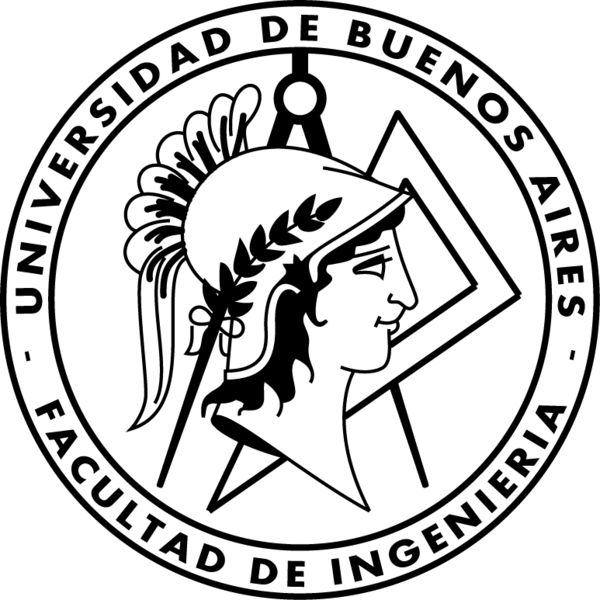
\includegraphics[width=7.5cm, height=7.5cm]{images/logo}
    \end{center}

    \materia{Organización de Datos}
    \submateria{Segundo Cuatrimestre 2017}
    \titulo{Trabajo Práctico 1}

    \integrante{Rodrigo De Rosa}{97799}{rodrigoderosa@outlook.com}
    \integrante{Marcos Schapira}{97934}{schapiramarcos@gmail.com}
    \integrante{Facundo Guerrero}{97981}{facundoiguerrero@gmail.com}
    \maketitle
    %Fin caratula
    %Table of contents
    \newpage
    \pagenumbering{roman}
    \tableofcontents
    %Fin table of contents
    %Informe
    \newpage
	\pagenumbering{arabic}
	\part{Análisis de la variación de precio en el périodo 2013-2017}

		\section{Análisis Global}

      \subsection{Objetivo}

        Esta sección tiene el objetivo de analizar como fueron variando los precios de las distintas propiedades en los últimos 4 años. Con fin introductorio, se quiere brindar una mirada global acerca de la fluctuación de los precios de todas las propiedades a lo largo de los últimos 4 años.

        Dicha variación se considera sobre el precio aproximado de cada propiedad en $usd$. Cabe mencionar que el set de datos utilizado para este análisis solo contiene propiedades de \code{CABA+GBA} Ademas, como esta sección es una generalización, no se filtran los features por tipo de propiedad ni cualquier otra  característica.

      \subsection{Preparación y procesamiento de los datos}

        Para poder obtener una mejor visualización global de los datos, se tuvieron en cuenta algunas características sobresalientes para filtrar los datos. Como primera aproximación, se recortaron todos los features que no fueran
        de \code{CABA+GBA}. Por otro lado, se filtraron los features a los cuales no fue posible obtener el precio. Sumado a esto, también fueron filtrados los features a los cuales no se pudo obtener la ubicación geográfica.
        Por otra parte, cabe destacar que el análisis de la variación global que esta próximo a presentarse, fue realizado sobre el precio aproximado de cada propiedad en $usd$. Por último, al tratarse de una primera visión global, esta sección no presenta filtrado por ninguna característica adicional del set de datos.
        \\
        Para este el procesamiento de los datos, primero se separaron y agruparon los features por años. A continuación, para cada dataframe formado, es decir para las propiedades de un determinado año, lo que se hizo fue separarlas por meses. Entonces hasta el momento tenemos las propiedades separadas por años y por meses. Por último para cada año, se agruparon todas las propiedades de un mismo mes dejando como valor el precio en dolares promedio de las mismas.

      \subsection{Presentación de los gráficos de promedios}

        Aquí se muestran los gráficos que representan los promedios anteriormente mencionados para cada año.
        Vale aclarar que en los siguientes 5 gráficos el eje x representa los meses de cada año, y el eje y representa el precio de las propiedades en usd. Dicho precio varia entre 0$-$450000, para obtener una mirada objetiva de los gráficos que serán presentados acontinuación.

				\begin{center}
       				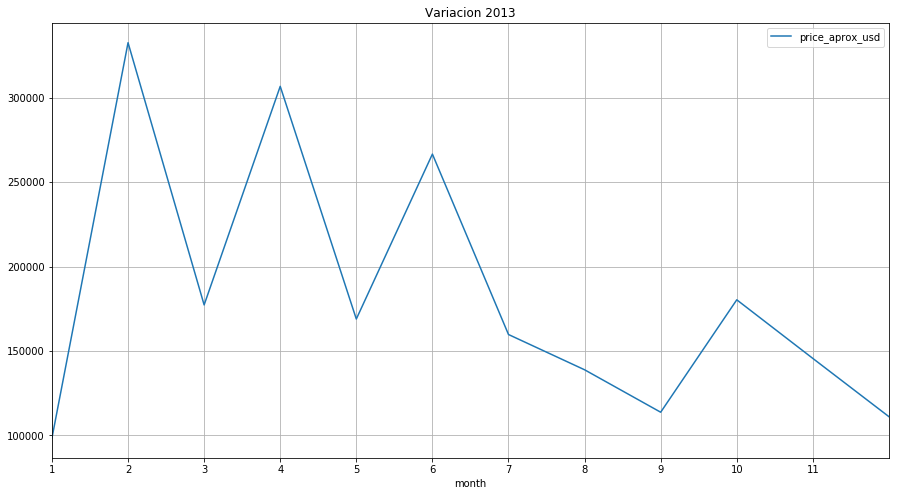
\includegraphics[width=6in, height=4.2in]{images/variacion2013}
		   	\end{center}
        \begin{center}
       				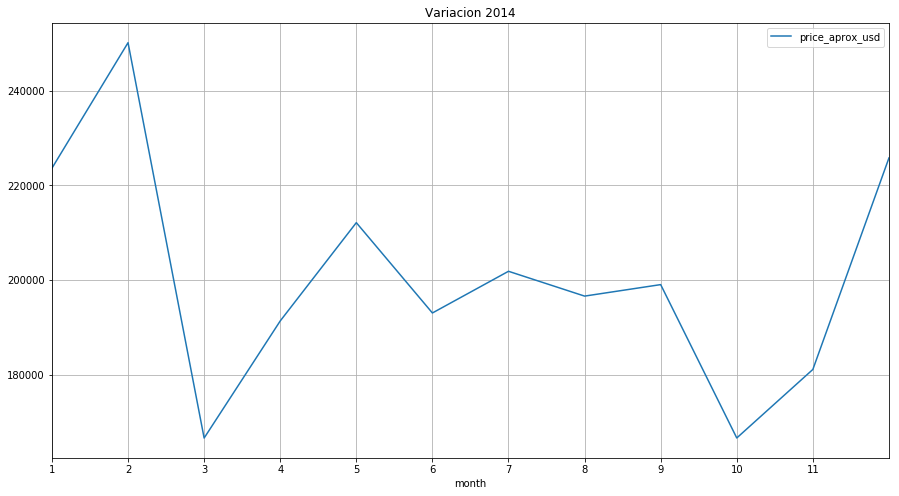
\includegraphics[width=6in, height=4.2in]{images/variacion2014}
		   	\end{center}
        \begin{center}
       				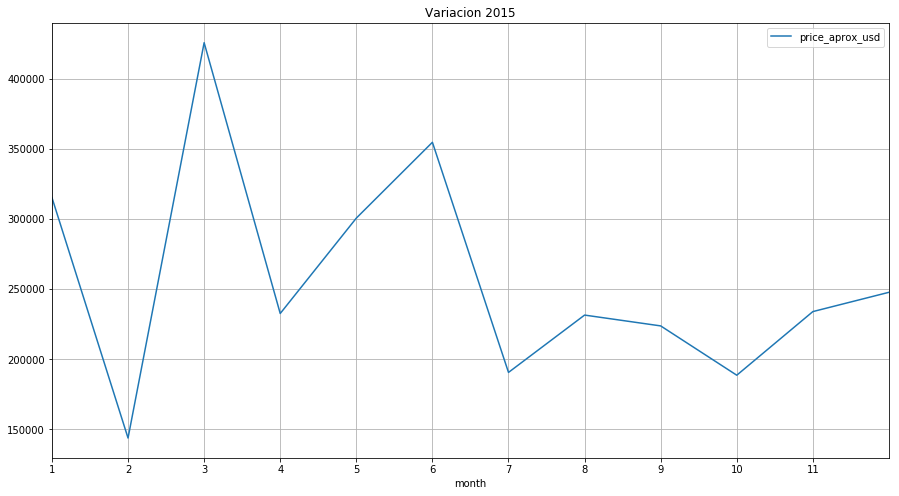
\includegraphics[width=6in, height=4.2in]{images/variacion2015}
		   	\end{center}
        \begin{center}
       				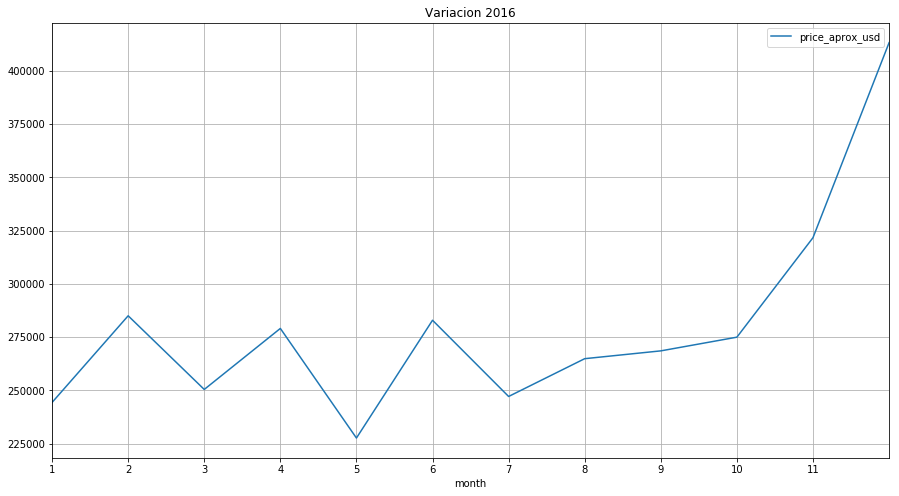
\includegraphics[width=6in, height=4.2in]{images/variacion2016}
		   	\end{center}
        \begin{center}
       				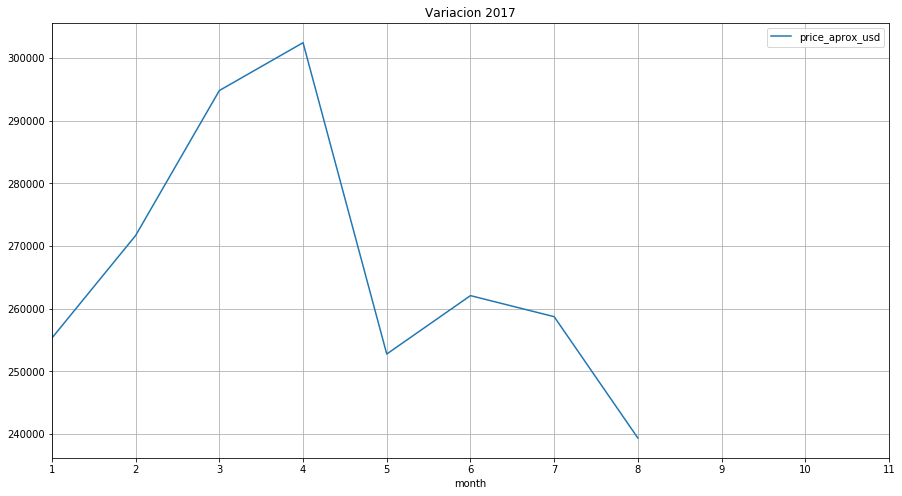
\includegraphics[width=6in, height=4.2in]{images/variacion2017}
		   	\end{center}

      \subsection{Ubicación de las propiedades}



      \subsection{Conclusiones}

      De los gráficos anteriormente presentados, podemos rápidamente obtener los meses con mayor y menor precio de propiedades en cada año:

      \begin{center}
        \begin{tabular}{ |c|c|c| }
          \hline
          \multicolumn{3}{|c|}{Limites de precios por años.}\\
          \hline
          \hline
          Año & Mes con Mayor Precio & Mes con menor Precio \\
          \hline
          2013 & Febrero & Enero \\
          2014 & Febrero & Marzo-Octubre \\
          2015 & Marzo & Febrero \\
          2016 & Diciembre & Mayo \\
          2017 & Abril & Agosto \\

          \hline
        \end{tabular}
      \end{center}

      Con el objetivo de poder apreciar la diferencia general entre los precios de distintos años, presentamos el siguiente gráfico:

      \begin{center}
            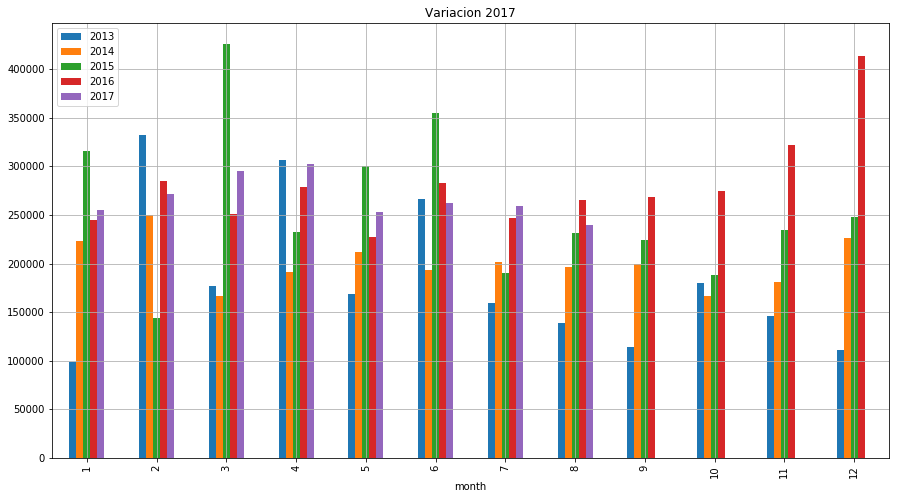
\includegraphics[width=6in, height=4.2in]{images/comparacionAnual}
      \end{center}

      Seguir obteniendo conclusiones en base al analisis que hagamos!!!!

      \subsection{Análisis dependiendo del tipo de propiedad}
      \tab Esta sección basa el análisis de la variación de los precios de los distintos tipos de propiedades, siendo estos: \code{$Casas$}, \code{$Departamentos$} y \code{$PH$}.

      \subsubsection{Preparación y procesamiento de los datos}
      La preparación de los datos para esta sección, es la misma que la de la sección anterior con el agregado de que inicialmente se filtra por 1 de los 3 tipos de propiedades mencionados anteriormente.

      \subsubsection{Análisis de la variacion de precios de las casas}

      Ahora vamos a presentar los graficos de los promedios por mes de cada año para las casas:
      \begin{center}
            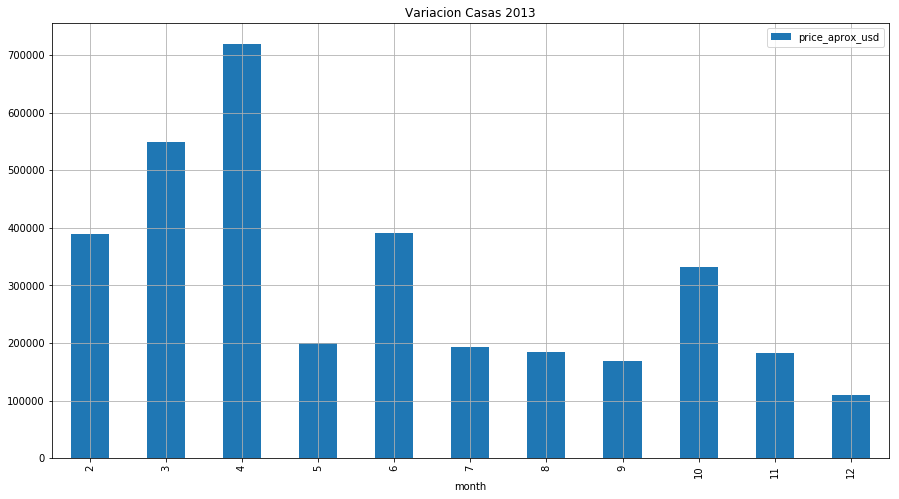
\includegraphics[width=6in, height=4.2in]{images/vCasas2013}
      \end{center}
      \begin{center}
            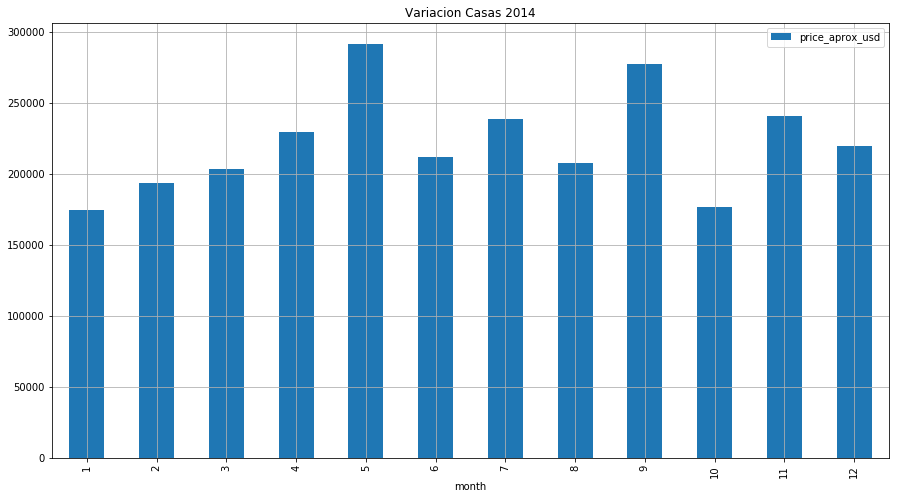
\includegraphics[width=6in, height=4.2in]{images/vCasas2014}
      \end{center}
      \begin{center}
            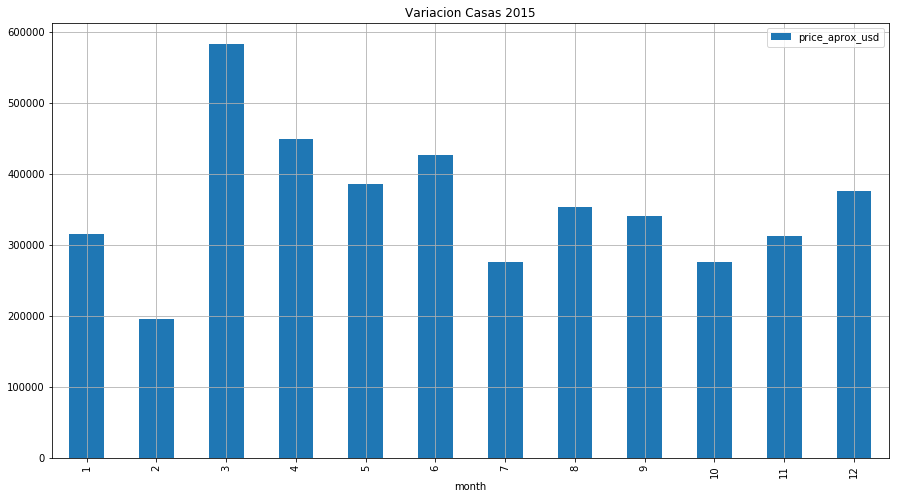
\includegraphics[width=6in, height=4.2in]{images/vCasas2015}
      \end{center}
      \begin{center}
            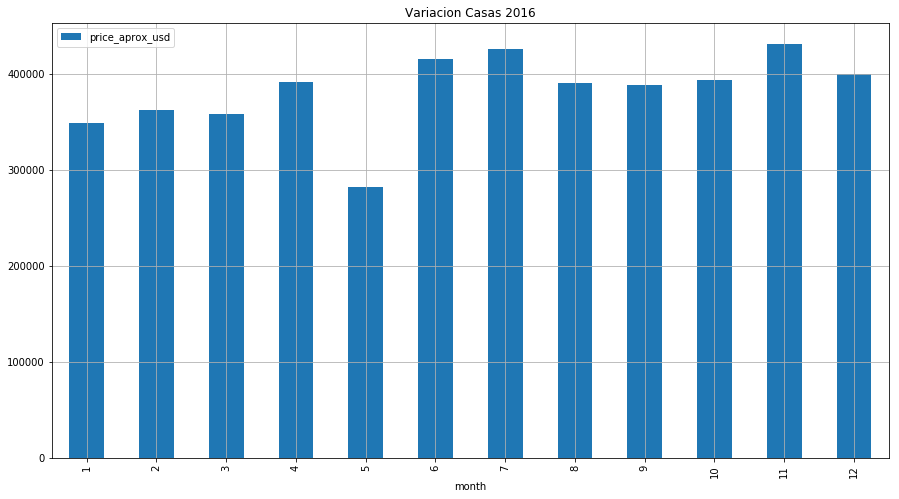
\includegraphics[width=6in, height=4.2in]{images/vCasas2016}
      \end{center}
      \begin{center}
            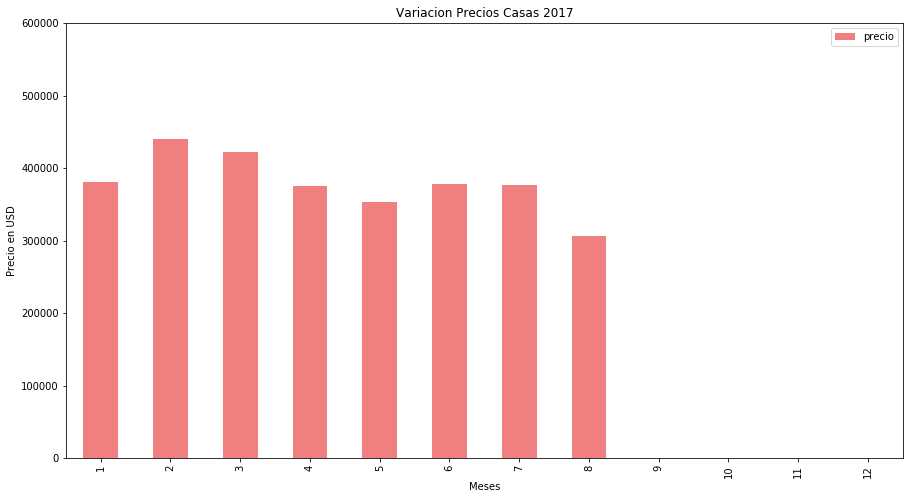
\includegraphics[width=6in, height=4.2in]{images/vCasas2017}
      \end{center}

      \subsubsection{Conclusiones de la variación de precios de las casas}

      Agregar conclusiones

      \subsubsection{Análisis de la variacion de precios de los departamentos}

      Aqui se van a añadir los graficos de los promedios por mes de cada año para los departamentos:
      \begin{center}
            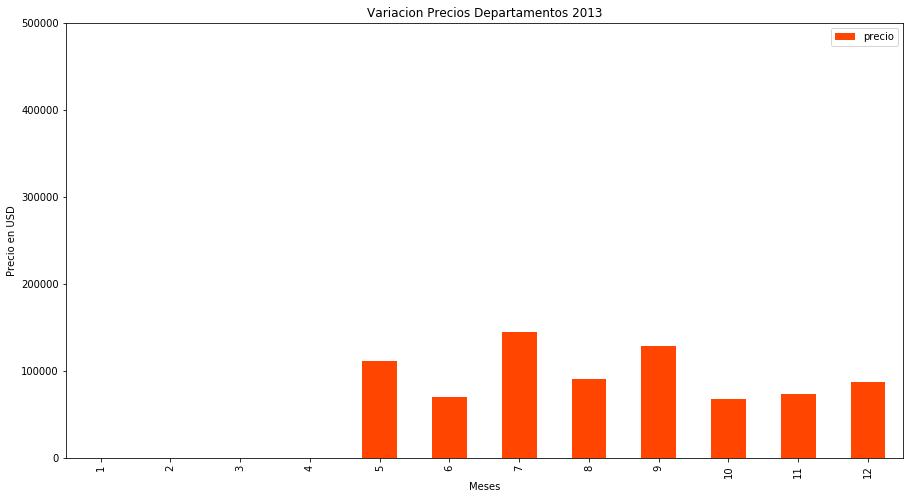
\includegraphics[width=6in, height=4.2in]{images/vDeptos2013}
      \end{center}
      \begin{center}
            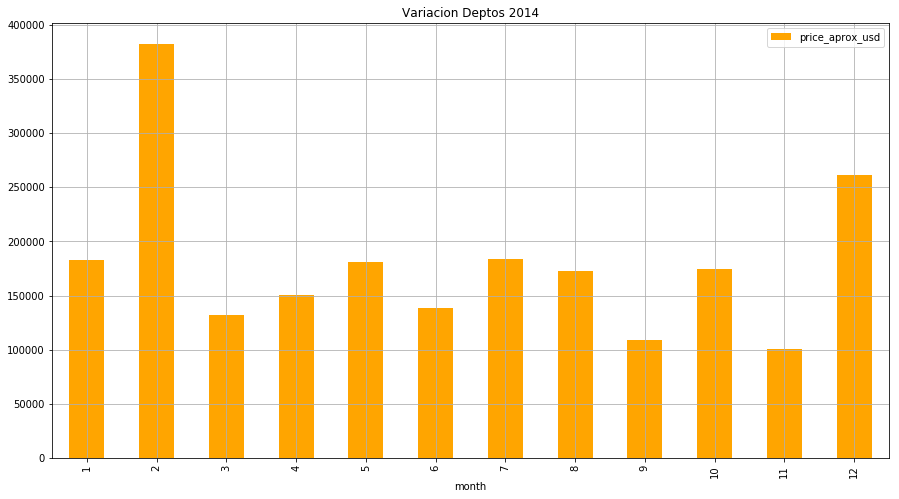
\includegraphics[width=6in, height=4.2in]{images/vDeptos2014}
      \end{center}
      \begin{center}
            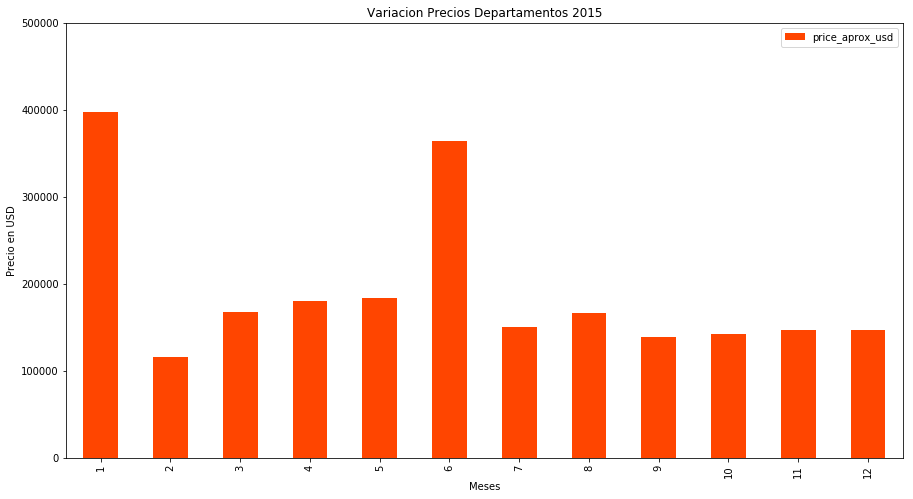
\includegraphics[width=6in, height=4.2in]{images/vDeptos2015}
      \end{center}
      \begin{center}
            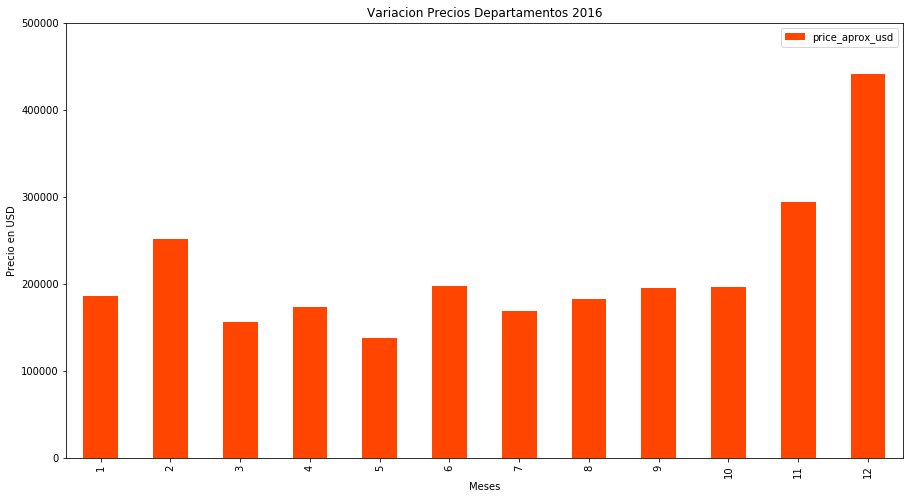
\includegraphics[width=6in, height=4.2in]{images/vDeptos2016}
      \end{center}
      \begin{center}
            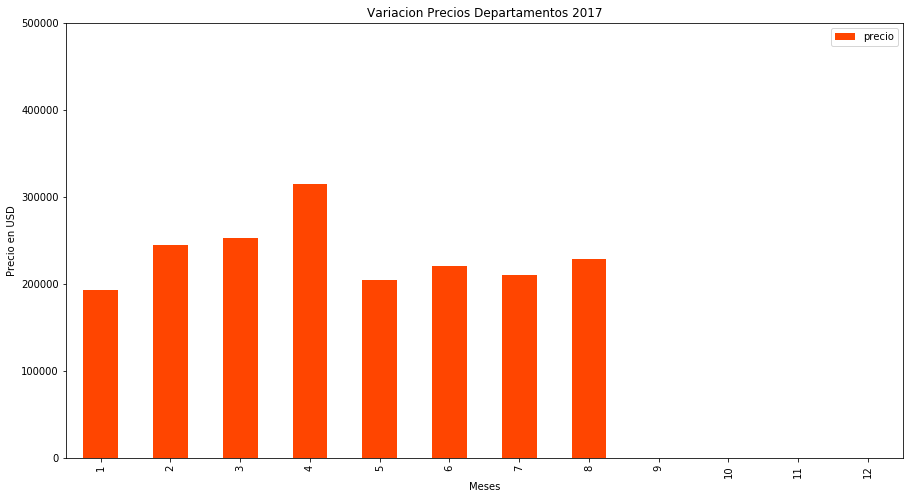
\includegraphics[width=6in, height=4.2in]{images/vDeptos2017}
      \end{center}

      \subsubsection{Conclusiones de la variación de precios de los departamentos}

      Agregar conclusiones

      \subsubsection{Análisis de la variacion de precios de los ph}

      Aqui se van a añadir los graficos de los promedios por mes de cada año para los departamentos:
      \begin{center}
            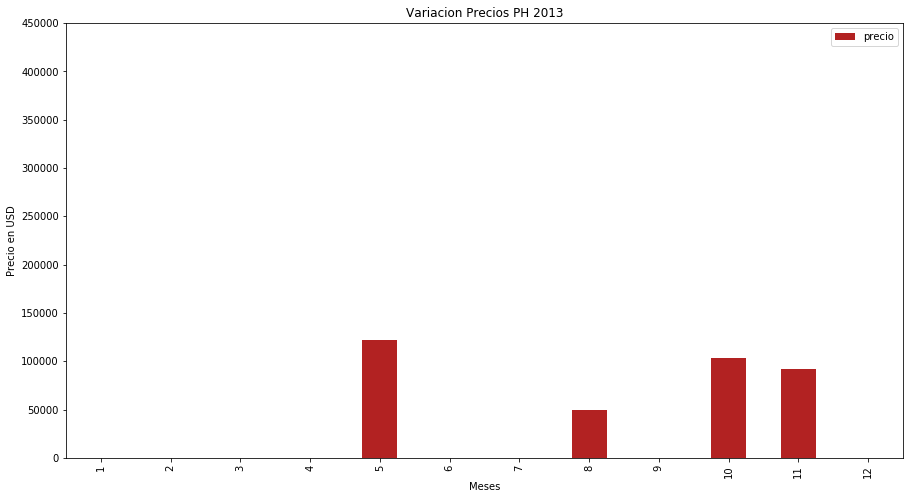
\includegraphics[width=6in, height=4.2in]{images/vPH2013}
      \end{center}
      \begin{center}
            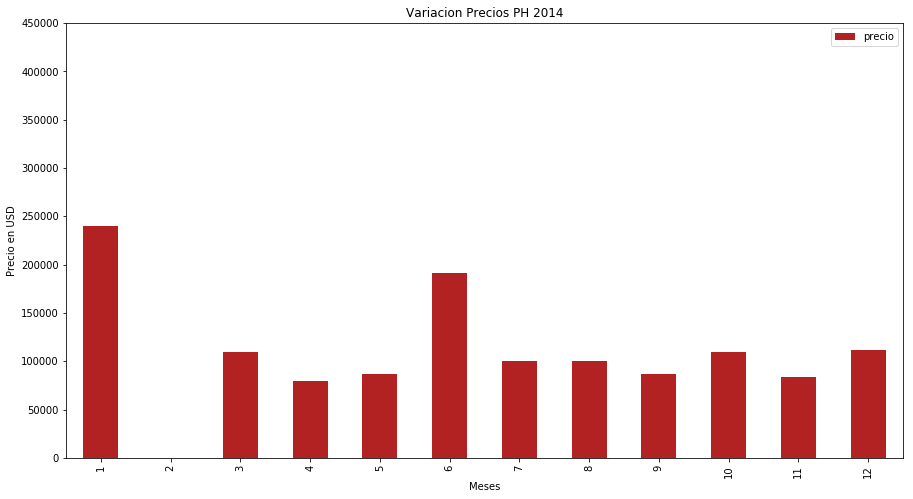
\includegraphics[width=6in, height=4.2in]{images/vPH2014}
      \end{center}
      \begin{center}
            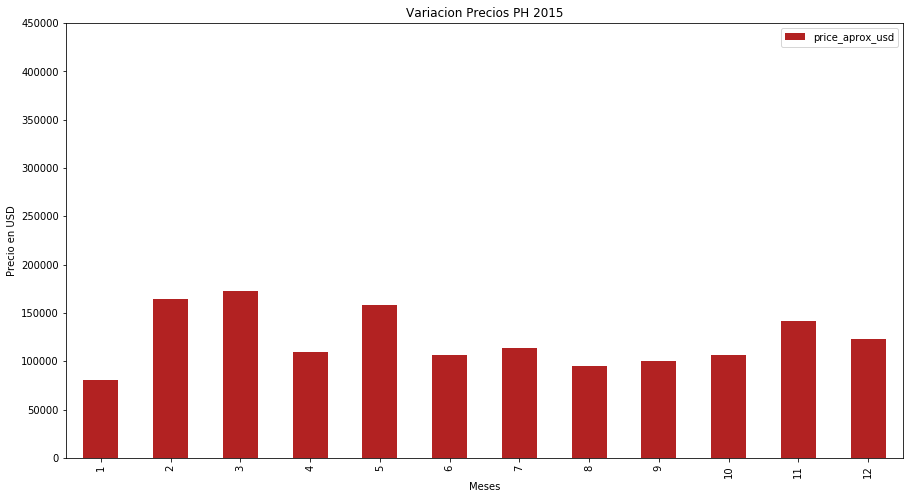
\includegraphics[width=6in, height=4.2in]{images/vPH2015}
      \end{center}
      \begin{center}
            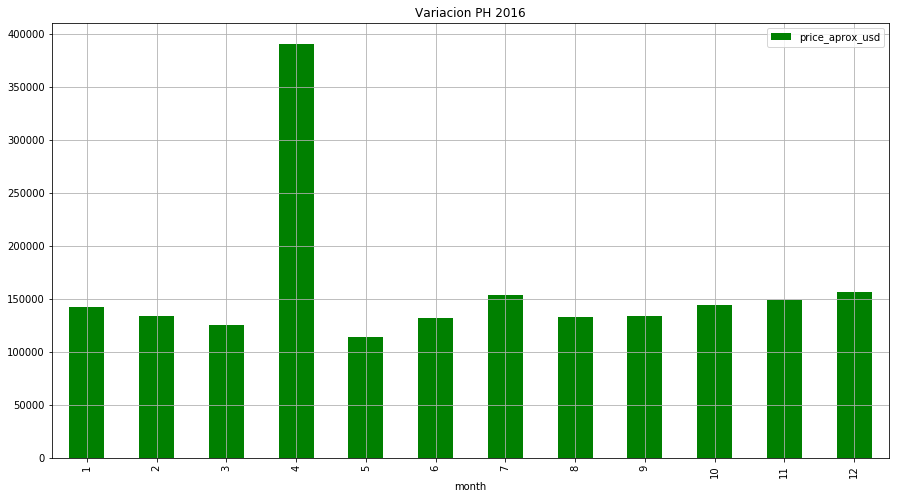
\includegraphics[width=6in, height=4.2in]{images/vPH2016}
      \end{center}
      \begin{center}
            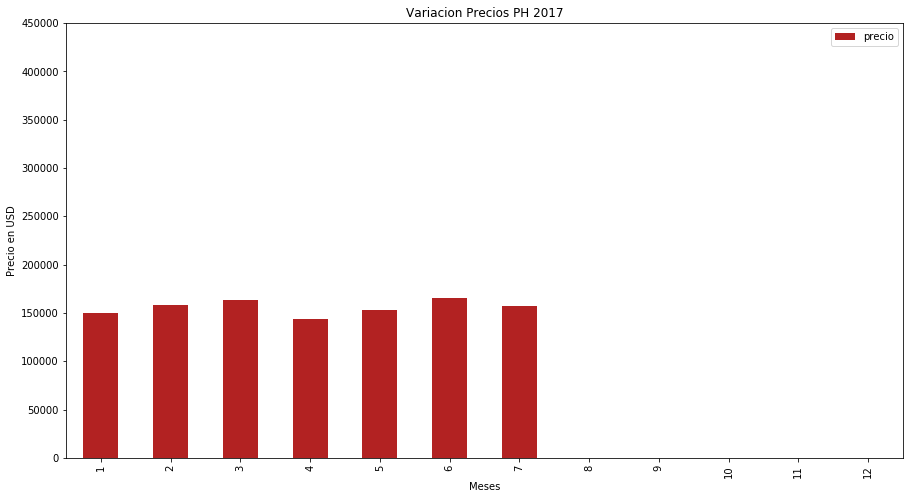
\includegraphics[width=6in, height=4.2in]{images/vPH2017}
      \end{center}

      \subsubsection{Conclusiones de la variación de precios de los departamentos}

      Agregar conclusiones

      \subsubsection{Conclusiones generales}

      Agregar conclusiones.

      Con motivo de representar cualitativamente la relacion entre los tipos de propiedades en los distintos años,
      presentamos el siguiente gráfico:

      \begin{center}
            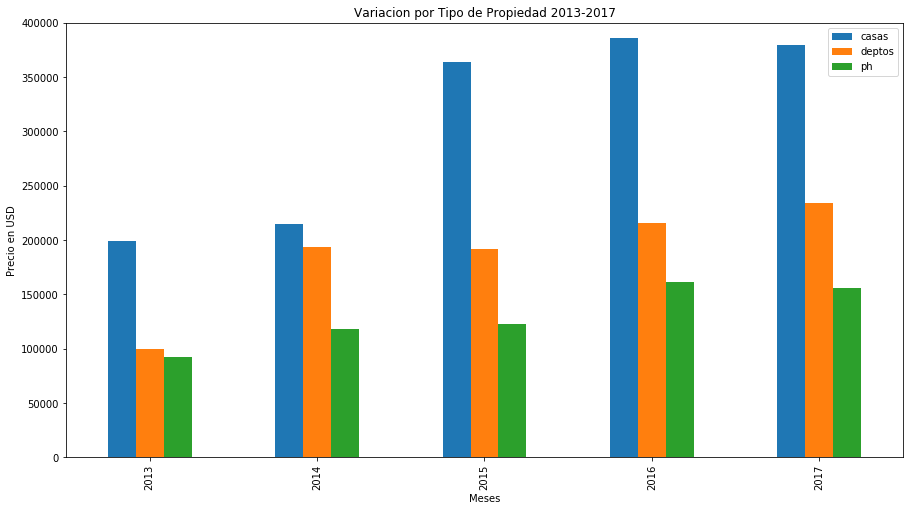
\includegraphics[width=6in, height=4.2in]{images/vTipoProp}
      \end{center}

      En el gráfico anterior se puede apreciar que las casas son las que tienen mayor precio promedio
      a lo largo de los años, seguidas por los departamentos y luego los ph.
      Ademas se puede apreciar que el año 2016 fue el año en donde las propiedades alcanzaron su mayor valor.
\end{document}
